\documentclass[polish,11pt,a4paper,twoside]{article}

\usepackage[utf8]{inputenc}
\usepackage[T1]{fontenc}
\usepackage[polish]{babel}
\usepackage[a4paper]{geometry}
\usepackage{listings}
\usepackage{graphicx}
\usepackage{amsthm}
\usepackage{color}
\usepackage{xcolor}
\usepackage{caption}
\usepackage{hyperref}
\usepackage{fancyhdr}

\lstset {
language=Java,
captionpos=t,
tabsize=2,
frame=lines,
keywordstyle=\color{blue},
commentstyle=\color{gray},
stringstyle=\color{red},
numbers=left,
numberstyle=\tiny,
numbersep=5pt,
breaklines=true,
showstringspaces=false,
basicstyle=\footnotesize,
emph={label}
}
\DeclareCaptionFont{white}{\color{white}}
\DeclareCaptionFormat{listing}{\colorbox{gray}{\parbox[c][0.25cm]{\textwidth}{#1#2#3}}}
\captionsetup[lstlisting]{format=listing,labelfont=white,textfont=white}

\geometry{verbose,tmargin=2cm,bmargin=2cm,lmargin=2cm,rmargin=2cm,headheight=2cm,headsep=2cm,footskip=1cm}

\begin{document}

\pagestyle{fancy}
\fancyhf{} % clear all header and footer fields
\fancyfoot[R]{\footnotesize \thepage}
\renewcommand{\headrulewidth}{0pt}
\renewcommand{\footrulewidth}{0pt}

\author{Bartłomiej Hyży\\Informatyka Stosowana, III rok\\WEAIiE, AGH}
\date{13.06.2011}
\title{Administracja sieciami lokalnymi -\\projekt sieci LAN}
\maketitle

\thispagestyle{fancy}

\section{Schemat sieci}
Poniższy schemat przedstawia zaprojektowaną przez nas sieć lokalną. Zbudowana jest ona z 5 podsieci, z czego tylko w 3 znajdują się hosty. Jedna podsieć podzielona jest dodatkowo na trzy sieci wirtualne (VLAN), zaznczone na rysunku kolorowymi prostokątami. Obok hostów i odpowiednich interfejsów routerów zaznaczono ich adresy. Dwie podsieci adresowane są jedynie w IPv6, jedna w IPv4. Dodatkowo pomiędzy routerami R1 i R3 utworzono tunel IPv4 przez który odbywa się komunikacji dwóch podsieci w IPv6. W następnych rozdziałach przedstawiono konfigurację zaprezentowanej sieci w oparciu o sprzęt sieciowy Cisco.
\begin{figure}[!htb]
  \begin{center}
    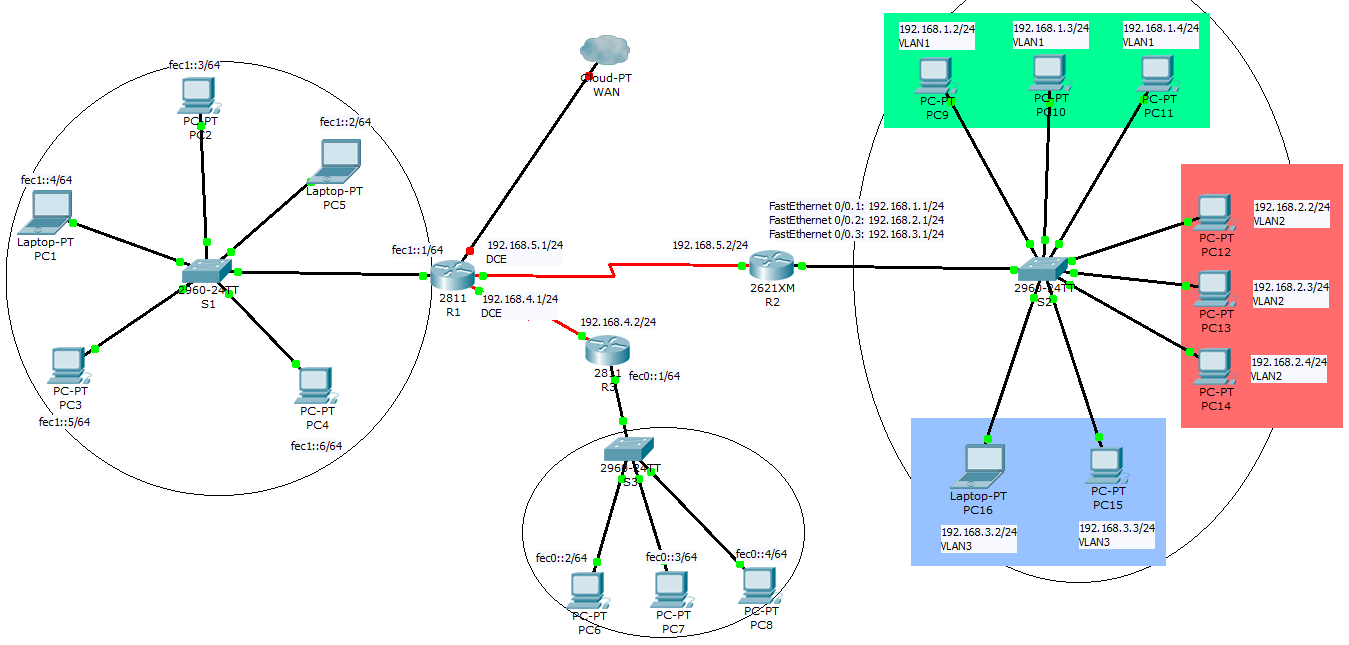
\includegraphics[width=0.9\textwidth]{schemat.png}
    \caption{Schemat budowy sieci LAN} \label{fig:schemat} 
  \end{center}
\end{figure}

\section{Wstępna konfiguracja sieci}
Pierwszym krokiem jest skonfigurowanie podstawowych ustawień routerów, switchy oraz hostów, takich jak adresy interfejsów czy sieci wirtualne.

\subsection{Konfiguracja routerów}

\subsubsection{Router R1}

Na poczatku wchodzimy w tryb uprzywilejowany:
\begin{lstlisting}
Router>enable
\end{lstlisting}
Następnie przechodzimy w tryb konfiguracji za pomocą terminala:
\begin{lstlisting}
Router#conf t
Enter configuration commands, one per line.  End with CNTL/Z.
\end{lstlisting}
Najpierw ustawiamy nazwę routera na bardziej informatywną:
\begin{lstlisting}
Router(config)#hostname R1
\end{lstlisting}
Kolejny krok to konfiguracja interfejsów routera. Najpierw konfigurowany jest interfejs serialowy pomiędzy routerem R1 a R3:
\begin{lstlisting}
! wybranie interfejsu do konfiguracji
R1(config)#interface Serial 1/0 
! przypisanie adresu IPv4
R1(config-if)#ip address 192.168.4.1 255.255.255.0 
! ustawienie czestotliwosci zegara lacza serialowego (koncowka DCE)
R1(config-if)#clock rate 128000 
! uruchomienie interfejsu
R1(config-if)#no shutdown 

%LINK-5-CHANGED: Interface Serial1/0, changed state to up

R1(config-if)#exit ! opuszczenie konfiguracji interfejsu
\end{lstlisting}
Analogicznie konfigurujemy interfejs serialowy 1/1 prowadzący do routera R2:
\begin{lstlisting}
R1(config)#interface Serial 1/1
R1(config-if)#ip address 192.168.5.1 255.255.255.0
R1(config-if)#clock rate 128000
R1(config-if)#no shutdown 

%LINK-5-CHANGED: Interface Serial1/1, changed state to up

R1(config-if)#exit
\end{lstlisting}
Jako ostatni konfigurowany jest interfejs FastEthernet 0/0, będący bramą dla podsieci po lewej stronie schematu:
\begin{lstlisting}
! uruchomienie konf. interfejsu FE0/0
R1(config)#interface FastEthernet 0/0
! usuniecie przypisanego adresu IPv4 
R1(config-if)#no ip address 
! przypisanie adresu IPv6 (brama podsieci)
R1(config-if)#ipv6 address fec1::1/64 
! aktywacja obslugi IPv6 na interfejsie
R1(config-if)#ipv6 enable 
! uruchomienie interfejsu
R1(config-if)#no shutdown 

%LINK-5-CHANGED: Interface FastEthernet0/0, changed state to up
\end{lstlisting}
Na końcu wychodzimy z trybu konfiguracji i zapisujemy wprowadzone ustawienia do pamięci urządzenia, dzięki czemu zostaną one odtworzone po ponownym uruchomieniu routera:
\begin{lstlisting}
R1(config-if)#Ctrl+C
R1#wr

Building configuration...
[OK]
\end{lstlisting}


\subsubsection{Router R3}
Konfiguracja routera R3 przebiega analogicznie jak w przypadku R1, z dokładnością do adresów interfejsów:
\begin{lstlisting}
Router>
Router>enable
Router#conf t
Enter configuration commands, one per line.  End with CNTL/Z.

Router(config)#hostname R3

R3(config)#interface serial 1/0
R3(config-if)#ip address 192.168.4.2 255.255.255.0
R3(config-if)#no shutdown 

%LINK-5-CHANGED: Interface Serial1/0, changed state to up

R3(config-if)#exit

R3(config)#interface FastEthernet 0/0
R3(config-if)#no ip address 
R3(config-if)#ipv6 address fe0::1/64
R3(config-if)#ipv6 enable
R3(config-if)#no shutdown 

%LINK-5-CHANGED: Interface FastEthernet0/0, changed state to up

R3(config-if)#

%SYS-5-CONFIG_I: Configured from console by console

R3#wr
Building configuration...
[OK]
\end{lstlisting}

\subsubsection{Router R2}
Konfiguracja routera R2 przebiega podobnie jak dla R1 i R3 w przypadku interfejsu serialowego. Różni się natomiast sposób, w jaki konfigurowany jest interfejs FastEthernet, z uwagi na fakt, że zdefiniowane muszą zostać 3 podinterfejsy stanowiące bramy dla sieci wirtualnych skonfigurowanych na switchu S2.
Najpierw przeprowadzamy konfigurację interfejsu serialowego 1/0, analogicznie jak w przypadku R1 i R3:
\begin{lstlisting}
Router>enable
Router#conf t
Enter configuration commands, one per line.  End with CNTL/Z.

Router(config)#hostname R2
R2(config)#interface serial 1/0
R3(config-if)#ip address 192.168.5.2 255.255.255.0
R2(config-if)#no shutdown 

%LINK-5-CHANGED: Interface Serial1/0, changed state to up
R2(config-if)#exit
\end{lstlisting}
Następnie przechodzimy do konfiguracji interfejsu FastEthernet 0/0:
\begin{lstlisting}
R2(config)#interface fastEthernet 0/0
! kasujemy przypisany do interfejsu adres IPv4, gdyz tylko podinterfejsy beda miec adresy jako bramy VLANow
R2(config-if)#no ip address
R2(config-if)#no shutdown 

%LINK-5-CHANGED: Interface FastEthernet0/0, changed state to up
R2(config-if)#exit
\end{lstlisting}
Kolejny krok to konfiguracja podinterfejsów FastEthernet 0/0, które służyły będą jako bramy sieci wirtualnych:
\begin{lstlisting}
R2(config)#interface FastEthernet 0/0.1
R2(config-subif)#
%LINK-5-CHANGED: Interface FastEthernet0/0.1, changed state to up
%LINEPROTO-5-UPDOWN: Line protocol on Interface FastEthernet0/0.1, changed state to up

! ustawienie trybu enkapsulacji pakietow dla VLANu 2 na dot1Q
R2(config-subif)#encapsulation dot1Q 2
! konfiguracja podinterfejsu - bramy VLAN1
R2(config-subif)#ip address 192.168.1.1 255.255.255.0
R2(config-subif)#no shutdown 
R2(config-subif)#exit

R2(config)#interface FastEthernet 0/0.2
R2(config-subif)#
%LINK-5-CHANGED: Interface FastEthernet0/0.2, changed state to up
%LINEPROTO-5-UPDOWN: Line protocol on Interface FastEthernet0/0.2, changed state to up

! ustawienie trybu enkapsulacji pakietow dla VLANu 3 na dot1Q
R2(config-subif)#encapsulation dot1Q 3
! konfiguracja podinterfejsu - bramy VLAN2
R2(config-subif)#ip address 192.168.2.1 255.255.255.0
R2(config-subif)#no shutdown 
R2(config-subif)#exit

R2(config)#interface FastEthernet 0/0.3
R2(config-subif)#
%LINK-5-CHANGED: Interface FastEthernet0/0.3, changed state to up
%LINEPROTO-5-UPDOWN: Line protocol on Interface FastEthernet0/0.3, changed state to up

! ustawienie trybu enkapsulacji pakietow dla VLANu 4 na dot1Q
R2(config-subif)#encapsulation dot1Q 4
! konfiguracja podinterfejsu - bramy VLAN3
R2(config-subif)#ip address 192.168.3.1 255.255.255.0
R2(config-subif)#no shutdown 
R2(config-subif)#exit
\end{lstlisting}
Na koniec zapisujemy sporządzoną konfigurację:
\begin{lstlisting}
R2(config-if)#

%SYS-5-CONFIG_I: Configured from console by console

R2#wr
Building configuration...
[OK]
\end{lstlisting}


\subsection{Konfiguracja switchy}
Wstępnej konfiguracji poddawany jest tylko switch S2, który obsługuje 3 sieci wirtualne dla hostów do niego podłączonych. Pierwszy etap konfiguracji VLANow odbyl sie podczas uruchamiania podinterfejsów (bram) na routerze R2, po jednym dla każdej sieci wirtualnej.
Dalsza konfiguracja switchy S2 oraz S1 i S3 zaprezentowana jest w następnych rozdziałach.

\subsubsection{Switch S2}

Rozpoczynamy od wstepnej konfiguracji, tj. przejścia tryb "config" oraz ustalenia nazwy urządzenia na S2 celem łatwiejszej identyfikacji:
\begin{lstlisting}
Switch>enable
Switch#conf t
Enter configuration commands, one per line.  End with CNTL/Z.
Switch(config)#hostname S2
\end{lstlisting}
Następnie przystępujemy do ustawienia sieci wirtualnych. Wybraliśmy przypisanie do VLANów na podstawie portów switcha, w związku z czym konieczne jest skonfigurowanie odpowiednich portów jako przynależnych do konkretnych sieci wirtualnych. Najpierw jednak należy ustawić port, który połączony jest z routerem R2 dokonującym przełączania pakietów łączem "trunk":
\begin{lstlisting}
S6(config)#interface fastEthernet 0/9
S6(config-if)#switchport mode trunk 

%LINEPROTO-5-UPDOWN: Line protocol on Interface FastEthernet0/9, changed state to down

%LINEPROTO-5-UPDOWN: Line protocol on Interface FastEthernet0/9, changed state to up
\end{lstlisting}
Następnie konfigurujemy sieci wirtualne, poprzez przypisanie im opisowych nazw:
\begin{lstlisting}
S2(config)#vlan 2
S2(config-vlan)#name VLAN1
S2(config-vlan)#exit
S2(config)#vlan 3
S2(config-vlan)#name VLAN2
S2(config-vlan)#exit
S2(config)#vlan 4
S2(config-vlan)#name VLAN3
S2(config-vlan)#exit
\end{lstlisting}
Wreszcie dokonujemy przypisania portów do konkretnych sieci wirtualnych, zgodnie ze schematem budowy sieci:
\begin{lstlisting}
S2(config)#interface fastEthernet 0/3
S2(config-if)#switchport access vlan 2
S2(config-if)#switchport mode access 
S2(config-if)#exit
S2(config)#interface fastEthernet 0/4
S2(config-if)#switchport access vlan 2
S2(config-if)#switchport mode access 
S2(config-if)#exit
(...)
S2(config)#interface fastEthernet 0/8
S2(config-if)#switchport access vlan 3
S2(config-if)#switchport mode access 
S2(config-if)#exit
S2(config)#interface fastEthernet 0/1
S2(config-if)#switchport access vlan 4
S2(config-if)#switchport mode access 
S2(config-if)#exit
S2(config)#interface fastEthernet 0/2
S2(config-if)#switchport access vlan 4
S2(config-if)#switchport mode access 
S2(config-if)#exit
\end{lstlisting}


\subsection{Konfiguracja tunelu IPv6 przez IPv4}
\section{Listy ACL}
\section{Konfiguracja routingu}
\section{NAT}
\section{DHCP}



\end{document}
